\chapter{Systemstruktur}
\label{cha:syst}
\section{Moduldiagramm}
\label{sec:usec}
%	-Systemstruktur/Moduldiagramm einfügen und kurz beschreiben
%		-Hinweis, dass es sich um eine erste Planung handelt!


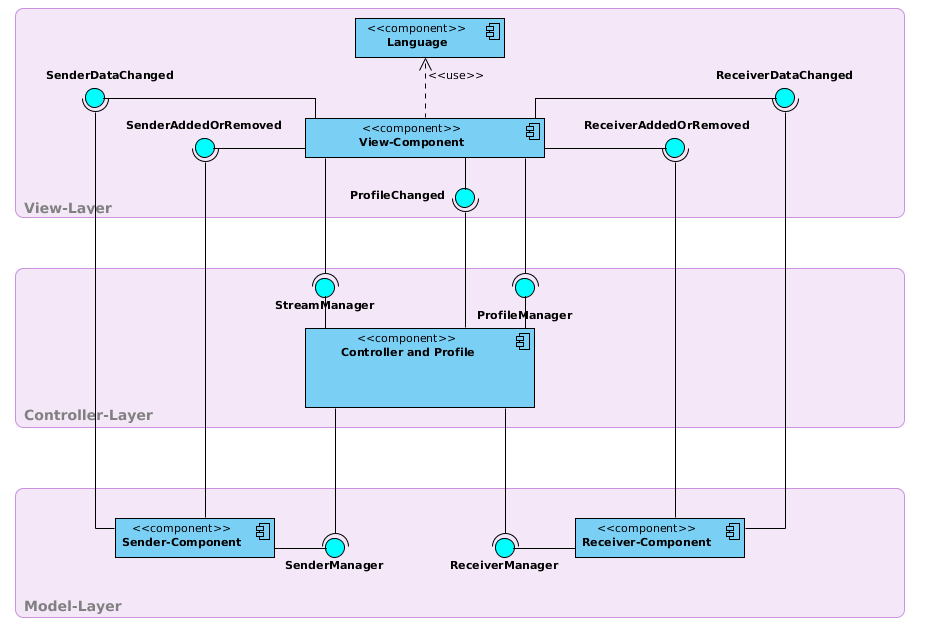
\includegraphics[width=15cm]{images/Overview.png}\\

Das Gesamtsystem wird zur besseren Verständlichkeit und zur Vermeidung von Abhängigkeiten 
in logische Komponenten unterteilt. Die grobe Grundstruktur gibt hierbei ein Model-View-Controller
Pattern vor. Dieses Pattern hat sich für die GUI Entwicklung zum quasi Standard herauskristallisiert. 
Das Konzept besteht darin, die Kopplung von der Benutzeroberfläche (View) und einer darunter stehenden Lösung des 
Problems so gering wie möglich zu halten. Diese darunter stehende Lösung des Problems wird dann wiederum in 
einen Controller und ein Model geteilt. Der Controller ist für die Initialisierung der Applikation zuständig und regelt die Kommunikation zwischen View und Model. 
In diesem Pattern weiß nur die View vom Model aber nicht umgekehrt. 
In dieser Applikation übernimmt der Controller die Verwaltung der Profile und informiert die View über die Sender und Empfangs
Komponente des Models. Das Model besteht aus einer Empfangs- und Sendekomponente. Beide können über den Controller
konfiguriert werden und beide Informieren über eventuelle Änderungen ihres Status über die SenderDataChanged
bzw. die ReceiverDataChanged Schnittstelle, welche mithilfe des Observer Pattern abonniert werden kann.
Die View-Komponente hat in dieser Applikation zwei Implementierungen und zwar
einerseits eine grafische Oberfläche (GUI) und ein Commandline Interface (CLI),
welches auch als Logger für die GUI dient. Um die Anforderung der Internationalisierung zu erfüllen, verfügt die Applikation zudem über eine Language
Komponente die für das Übersetzen von Nachrichten und Ausnahmen (Exceptions) verantwortlich ist.
Es wurden viele Ressourcen in die Erstellung dieser Komponenten Aufteilung des Systems gesteckt. 
Allerdings können sich im Laufe der Entwicklung immer unvorhersehbare Probleme auftun. In gravierenden Fällen
ist es möglich die Aufteilung über Change Requests an Probleme anzupassen.

\section{Daten Transfer Protokoll}
\label{sec:usec}

Um die Testbarkeit eines Multicast Netzwerkes zu ermöglichen, muss das Tool notwendigerweise
Datenpakete via Multicast versenden können. Die versendeten Pakete müssen Informationen über den
Zustand der Applikation zum Zeitpunkt des Versands beinhalten, um so beim Empfänger
Statistiken über die Übertragung erstellen zu können. Um die nötigen Informationen
zu strukturieren ist ein Datenformat von Nöten. Die Struktur sollte einfach
Erweiterbar und trotzdem simpel gehalten sein um das Dekodieren der Pakete 
effizient zu gestalten. Das TLV Protokoll erfüllt all diese Anforderungen.
TLV steht für Type-Length-Value-Format und wird in vielen vorhandenen 
Netzwerkprotokollen, wie zum Beispiel COPS, IS-IS, LLDP und RADIUS genutzt,
wobei es sich dort als erweiterbar und robust bewährt hat.
Bei diesem Protokoll wird jedes Attribut eines Paketes durch folgendes Tripel übermittelt:

\begin{itemize}
 \item[-] Type: bestimmt den Typ des Attributes, in unserem Fall ein unsinged 
                16bit Integer.
 \item[-] Length: bestimmt die Länge des Attribut Wertes und ist 
                  in unserem Fall ein unsigned 32bit Integer.
 \item[-] Value: enthält den eigentlichen Wert des Attributes.
\end{itemize}

Durch die einheitliche Struktur des Protokolls ist es sehr einfach Sequenzen von
TLV Tripel mit einer einheitlichen Funktion zu durchsuchen.
Hierbei werden Tripel mit einem unbekannten Typen ignoriert, was zu einer 
einfachen Erweiterbarkeit führt. Die Anzahl der Tripel im Paket muss nicht 
angegeben werden, da die Länge des Paketes schon im UDP Header enthalten ist.
Zudem kümmert sich UDP auch um die Integrität der Daten, ein extra CRC Hash oder
Paritybits müssen also nicht mit übertragen werden.
\\ \\
Um das hier spezifizierte Protokoll vom Hirschmann-Protokoll und anderen
Protokollen zu unterscheiden, ist ein Header vor den TLV Attributen wichtig. Daher muss vor dem ersten TLV Trippel 
folgendes Hexadezimales Bytemuster stehen.
\\ \\
05 39 00 00 00 00
\\ \\
Diesen Header kann man auch als TLV Trippel mit dem Typ 1337, der Datenlänge
0 und keinen Nutzdaten auffassen. Dieser Umstand vereinfacht potentiell das parsen des Protokolls.
\\ \\
\textbf{Das Protokoll kann wie folgt als DD dargestellt werden:} \\ \\
Paket = Header + {TLV} \\
Header = 0x053900000000 \\
TLV = Type + Length + Value  \\
Type = 0..65535  \\
Length = 0..4294967295 \\
Value = Datenstrom der zuvor genannten Länge. \\
\\ 
\begin{table}[htdp]
\centering
\caption{Im Protokoll verwendete Attribute}
\label{tab:prot}
\begin{tabular}{|l|l|p{9.5cm}|}
\hline
\textbf{Beschreibung} & \textbf{Typ} & \textbf{Attribut Wert} \\
\hline
Sender ID & 1 & Signed 32bit Integer Sender ID.\\
\hline
Eingestellte Paketsenderate & 2 & Pakete pro Sekunde als unsigned 32 bit Integer. \\
\hline
Ermittelte Paketsenderate & 3 & Pakete pro Sekunde als unsigned 32 bit Integer. \\
\hline
Sequenznumber & 4 & Signed 32bit Integer Sequenznumber. \\
\hline
Absendezeit & 5 & Nanosekunden seit dem 1. Januar 1970 00:00 Uhr UTC (vergleiche Unixzeit) als signed 64 bit Integer. \\
\hline
Daten & 6 & Datenstream variabler Länge. \\
\hline
\end{tabular}
\end{table}



